\documentclass{beamer}
\usepackage{algpseudocode}
\renewcommand{\vec}{\mathbf}
\usepackage[utf8]{inputenc}
 \usetheme{Boadilla}
 \usepackage{ragged2e}
\justifying
%Information to be included in the title page:
\title{Software Clusterings with Vector Semantics and the Call Graph}
\author[Marios Papachristou]{Marios Papachristou \\ \small \url{papachristoumarios@gmail.com} \\ \small \url{el15101@mail.ntua.gr}}

\institute[BaLab]{BALab, Athens University of Economics and Bussiness \\ National Technical University of Athens \\ Advisor: Prof. Diomidis Spinellis}
\date[ESEC/FSE 2019 SRC]{Student Research Competition \\ ESEC/FSE August 2019 \\ Estonia}
 
 
 
\begin{document}
 
\frame{\titlepage}
 
\begin{frame}
\frametitle{Problem Statement}

\begin{itemize}
    \item<1-> The architecture of a software system is the most fundamental realization of it
    \item<2-> When there is no specific definition of it, we can attempt to recover it
    \item<3-> One particular problem is the \textbf{clustering of its components into modules} 
    \item<4-> Many methods exist in literature
\end{itemize}


\end{frame}

\begin{frame}
\frametitle{Our motivation}

Our motivation, through this work is to 

\begin{enumerate}
    \item<1-> Provide a method for software clusterings through \textbf{vector semantics} and the \textbf{call graph}
    \item<2-> Evaluate our method on the \textbf{Linux Kernel Codebase}

    \item<3-> Compare it against state-of-the-art methods (ACDC \cite{acdc}, LIMBO \cite{limbo}) and agglomerative clustering methods (agglomerative clustering \cite{average, complete, ward}) 
\end{enumerate}
    
\end{frame}

\begin{frame}[allowframebreaks]
\frametitle{Our approach}

We took a simple approach to the problem
\begin{enumerate}
    \item Define the initial ``grains'' of the system. With the term ``grains'' we can refer e.g. to source files (.c), source (.c) and header (.h) files (combined) as well as one-top directory modules. 
    \item Preprocess the files attributed to the ``grains''
    \item Train a Skip-Gram model (Doc2Vec \cite{doc2vec}) on them and obtain vector representations of the ``grains'' $\vec x_1, \dots, \vec x_n$
    \item Generate the call graphs of the system using a static code analyzer (e.g. CScout \cite{cscout})
    
    \framebreak
    \item Put weights on the graph minor $H(V, E)$ induced by the ``grains'' as the normalized cosine similarities between them $$w(i, j) = \frac {1 + \cos(\vec x_i, \vec x_j)} 2 \qquad \forall (i, j) \in E(H)$$
    
    \item Run Louvain Community Detection on $H$ and obtain software clusterings
\end{enumerate}
    
\end{frame}

\begin{frame}{Preprocessing}

\begin{enumerate}
    \item First the code is tokenized and identifiers are split into their constituent parts using dynamic programming and n-grams. Stop-words are removed. 
    
    \item For example \texttt{zone\_seqlock\_init} becomes \texttt{zone}, \texttt{seqlock}, \texttt{init} and \texttt{inprogress} becomes \texttt{in} and \texttt{progress}
    
    \item Let $L(m)$ be the cost of the optimal split in the $m$-th character of the identifier. Then 

    $$\small L(m) = 
    \begin{cases}
	0 & m = 0 \\
	\min_{n \le \ell \le m - n} \{ L(\ell) + c(\ell, \ell + n) \} & \text{else} 
	

\end{cases}
$$

	\item The resulting tokens are lemmatized using the English Lemmatizer provided by the spaCy \cite{spacy} package

\end{enumerate}



\end{frame}

\begin{frame}{Embeddings}

A Skip-Gram model is trained. The objective of such a model is to maximize the probability that a word appears in a window (context) of size $2k + 1$

$$\frac {1} {N} \sum_{t = k}^{N - k} \log \Pr [w_t \mid w_{t-k}, \dots, w_{t + k}]$$

where 

$$\Pr [w_c \mid w_t] = \frac {\exp(s(w_c, w_t))} {\sum_{j = 1}^{V} \exp(s(w_t, j)}$$

We have used Doc2Vec for our training which extends the aforementioned idea to extract document embeddings.
    
\end{frame}

\begin{frame}{The Linux Kernel Codebase}
    \begin{itemize}
        \item A \textbf{HUGE} codebase consisting of $\sim$20.3 million lines of source code
        \begin{figure}
            \centering
            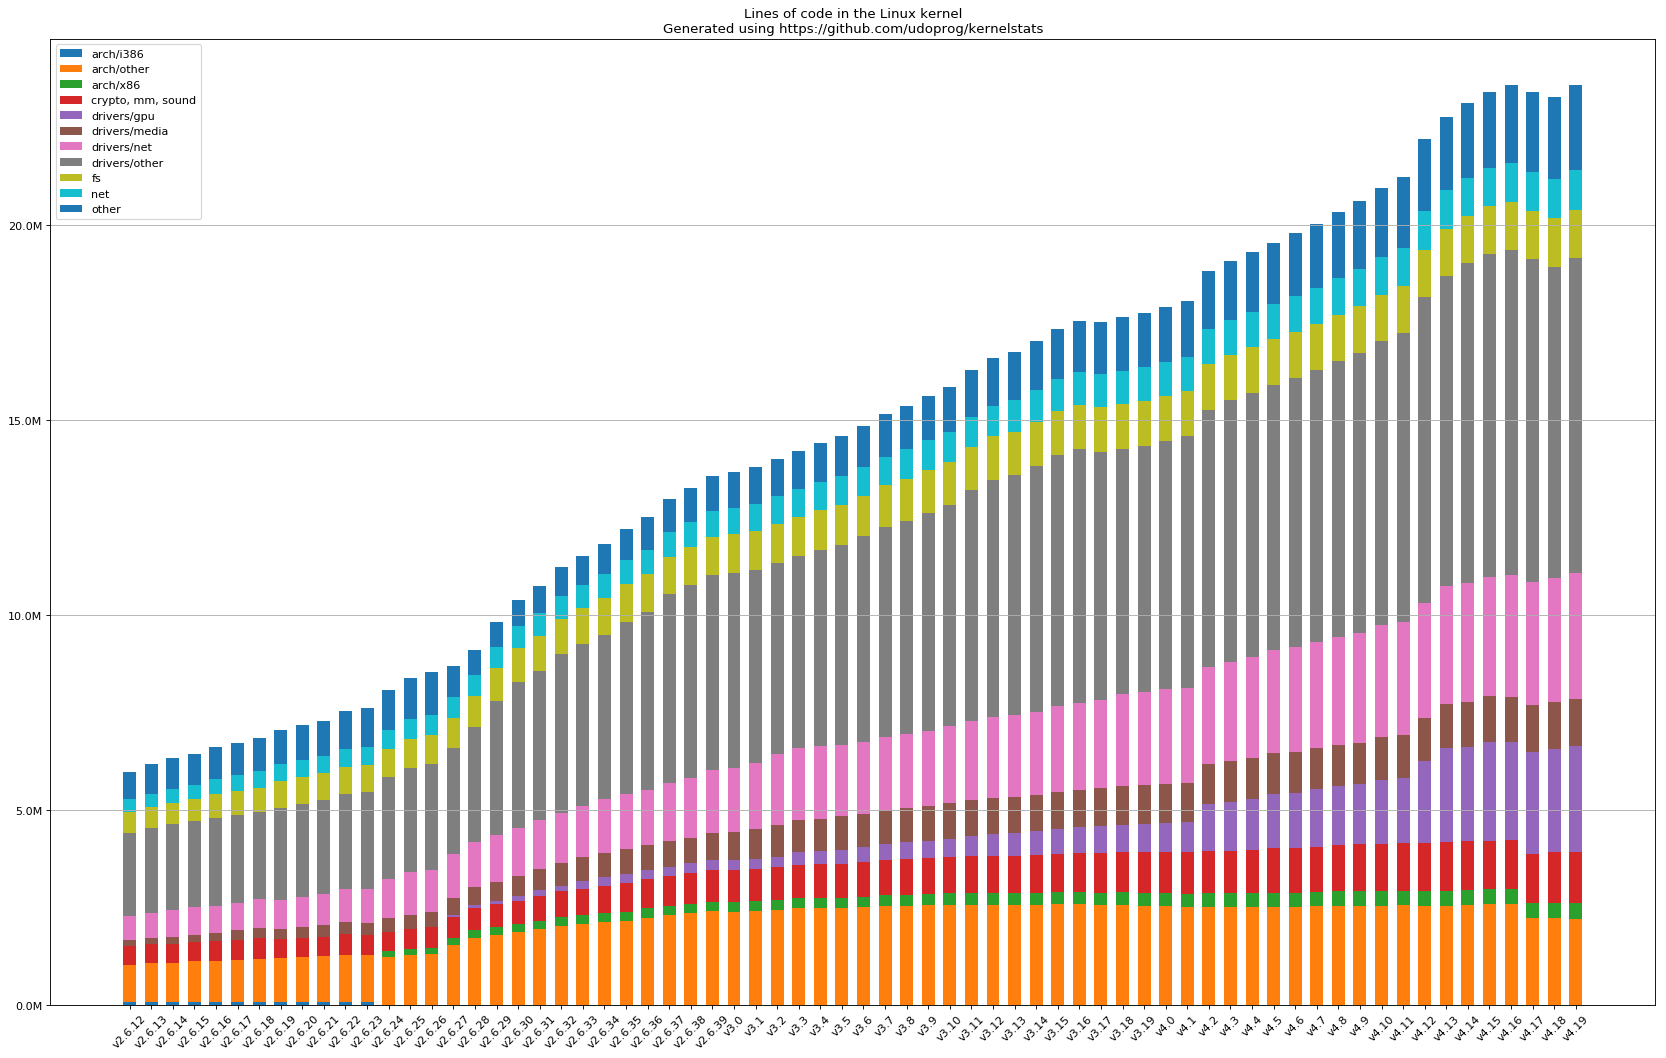
\includegraphics[scale=0.15]{linux.png}
            \caption{Linux Kernel Codebase Size over time. Source: Reddit}
            \label{fig:linux}
        \end{figure}
        
        \item Constantly growing
        \item Easy-to-find ground truth for evaluation
    \end{itemize}
    
    
\end{frame}

\begin{frame}[allowframebreaks]{Call Graphs}

The call graphs were extracted with CScout \cite{cscout} and are of the following forms

\begin{enumerate}
    \item Macro and Function Call Graph
    \item Control Dependency Graph 
    \item File include Graph
    \item Compile-time Dependency Graph
    \item Data dependency Graph (through globals)
    
\end{enumerate}

The extraction of the call graphs took $\sim 10$h and required $\sim 32$GB of RAM on a Debian server. 

\framebreak

\begin{figure}
    \centering
    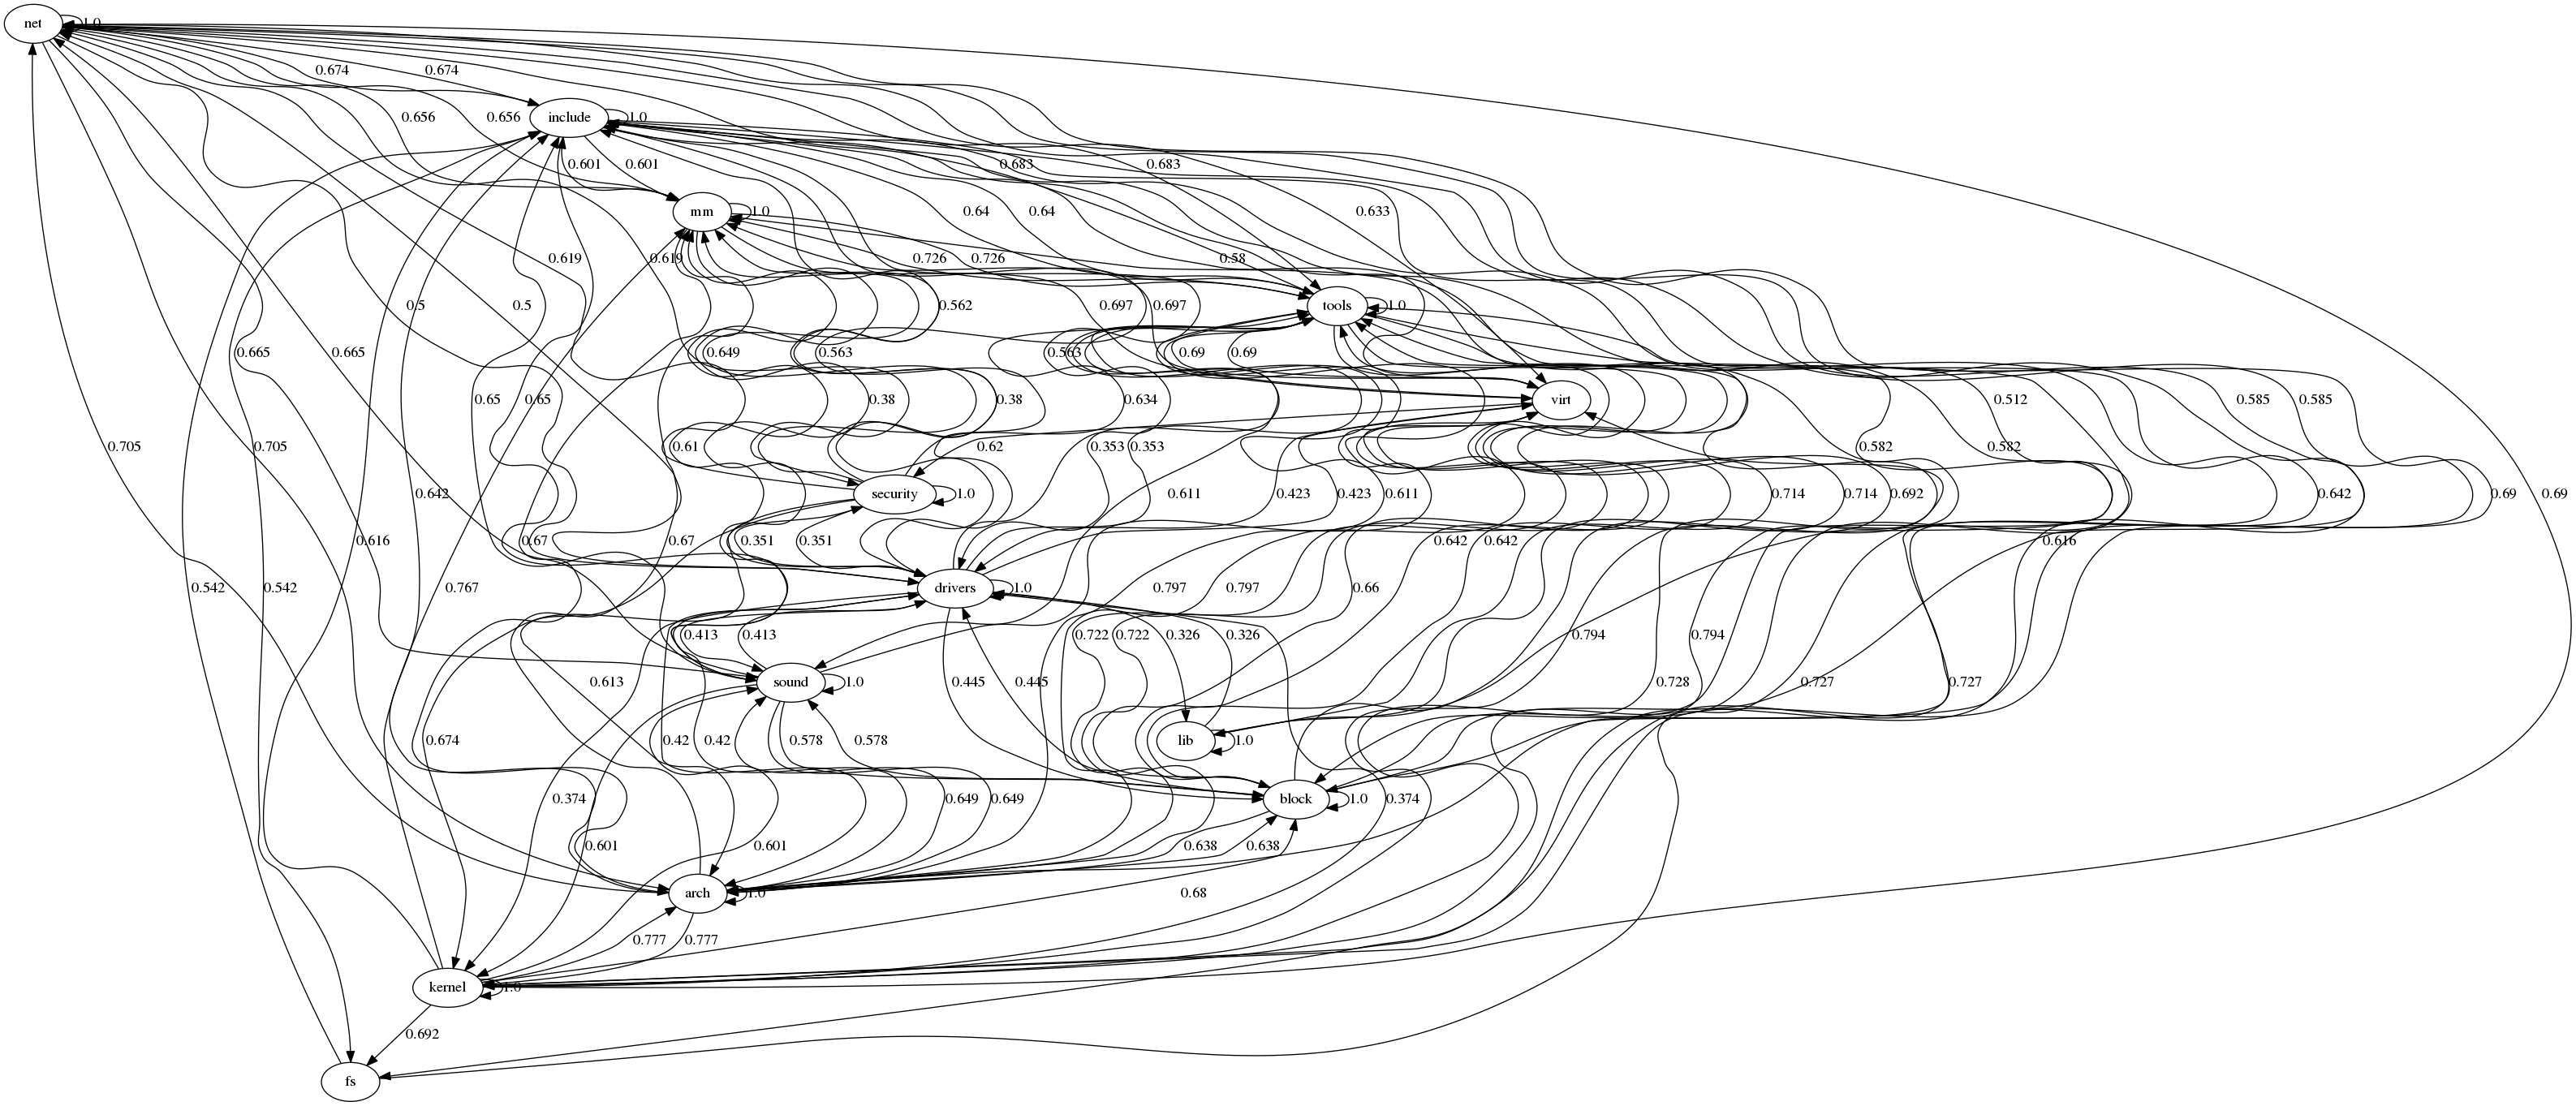
\includegraphics[keepaspectratio,width=0.9\paperwidth,                          height=\paperheight]{call_graph.png}
    \caption{Call Graph Example between Kernel one-level directories}
    \label{fig:my_label}
\end{figure}

% TODO How cscout operates? 

\end{frame}

\begin{frame}{Preparing the graph for clustering}

\begin{itemize}
    \item The weights assigned to every edge are the normalized cosine similarities
    $$\cos(\vec x_i, \vec x_j) = \frac {\langle \vec x_i, \vec x_j \rangle} {\| \vec x_i \| \| \vec x_j \|}$$
    $$w(i, j) = \frac {1 + \cos(\vec x_i, \vec x_j)} {2} \qquad \forall (i, j) \in E(H)$$
    
    \item Experiments were run using both the directed and the undirected version of the graph. The directed version of the graph required doing a bipartite transformation \cite{malliaros} where every edge $(i, j)$ was mapped to $\{ i, j' \}$ where $j'$ was a copy of $j \in V$. After community detection, the communities which $j$ and $j'$ belonged to were merged using a union-find data structure.  
    
\end{itemize}

\end{frame}

\begin{frame}[allowframebreaks]{Louvain Community Detection}

\begin{itemize}
    \item The Louvain method for community detection aims to produce communities which maximize the modularity function 
    
    $$Q(H) = \frac {1}{2m} \sum_{(i, j) \in E(H)} \left ( w(i, j) - \frac {k(i) k(j)} {2m} \right )$$
    
    where $m = \sum_{(i, j) \in E} w(i,j)$ and $k(i) = \sum_{j \in \mathrm{in}(i)} w(i, j)$ . 
    
    \item \textsc{modularity-optimization} is NP-Hard \cite{modularity}.
    \item The Louvain algorithm progresses agglomeratively by checking for each node $i$ where the largest change in $\Delta Q (i, j) $ occurs for each $j$ of its neighboring communities. 
    \framebreak
    
    \item The change $\Delta Q(i, j)$ in modularity is derived as 
        
    \small {
    $$ \Delta Q = \bigg[ \frac{\Sigma_{in} + 2k_{in} (i)}{2m} - \bigg(\frac{\Sigma_{tot} + k(i)}{2m}\bigg)^2 \bigg]-\bigg[\frac{\Sigma_{in}}{2m} - \bigg(\frac{\Sigma_{tot}}{2m}\bigg)^2-\bigg(\frac{k(i)}{2m}\bigg)^2\bigg] $$
    }
        
    
    where $\Sigma_{in}$ is sum of all the weights of the links inside the community $i$ is moving into, $\Sigma_{tot}$ is the sum of all the weights of the links to nodes in the community $i$ is moving into, $k_{in} (i)$ is the sum of the weights of the links between $i$ and other nodes in the community that $i$ is  moving into.
    
    \item The communities that Louvain Clustering produces 
    
\end{itemize}

\end{frame}

\begin{frame}{The MoJo Clustering Distance}

The MoJo \cite{mojo} metric is a clustering distance metric used for comparing software clusterings. The MoJo distance between two clusterings $\mathcal C_1, \mathcal C_2$ is defined as the minimum number of moves and joins to transform one clustering to another where 
\begin{itemize}
    \item \textbf{Move:} Moving a resource from one cluster to another (that includes moving a resource into a previously nonexistent cluster or creating a new cluster.
    \item \textbf{Join:} Join two clusters into one.
\end{itemize}

$$\textrm{MoJo} (\mathcal C_1, \mathcal C_2) = \min \{ \textrm{mno} (\mathcal C_1, \mathcal C_2), \textrm{mno}(\mathcal C_2, \mathcal C_1) \}$$
    Exact computation is not \textbf{efficient} so a \textbf{heuristic} is proposed.
\end{frame}


\begin{frame}[allowframebreaks]{Agglomerative Clustering}

\begin{block}{Idea}
    In every iteration pick two points/vertices $u$ and $v$ that maximize a linkage function and merge them together.
\end{block}



\begin{block}{Algorithm}

    \begin{algorithmic}
    \Function{AgglomerativeClustering}{$w, L, m, \vec x_1, \dots, \vec x_n$}
        \State $\mathcal C_0 \gets \{ \{\vec x_1, \}, \dots, \{ \vec x_n \}\}$
        \For {$1 \le t \le m$}
            \State $(\hat A, \hat B) \gets \mathrm {argmax}_{A, B \in \mathcal C_{t -1}} L(|A|, |B|, w(A, B)) $
            \State $\mathcal C_t \gets \mathcal C_{t - 1} \setminus \{ \{ \hat A \} , \{  \hat B \} \} \cup \{ \{ \hat A \cup \hat B \} \}$
        \EndFor
        \State \Return $\mathcal C_m$
    \EndFunction
  \end{algorithmic}

\end{block}

\framebreak

Linkage functions vary

\begin{itemize}
    \item Average Linkage $\mathrm{argmax}_{A, B} \frac {w(A, B)}{|A||B|}$
    \item Complete Linkage $\mathrm{argmax}_{a \in A, b \in B} w(a, b)$
    \item Single Linkage $\mathrm{argmin}_{a \in A, b \in B} w(a, b)$
    \item Ward Linkage 
    \item Information Loss (Agglomerative Information Bottleneck Algorithm)
\end{itemize}

The affinity function $w$ can be any distance measure. In our comparison, we have used the cosine distance affinity measure between the document embeddings.

\end{frame}


\begin{frame}{Main Software Clustering Algorithms}

The two main algorithms appearing in literature \cite{maqbool_overview, large_study} are 

\begin{itemize}
    \item LIMBO. An Information-Theoretic Clustering Algorithm based on the Agglomerative Information Bottleneck. The initial clusters are put on a B+-tree variant (DCF Tree) and then the leaves of the tree become the input of the Agglomerative Information Bottleneck Algorithm. 

    \item ACDC. TODO
    
\end{itemize}


    
\end{frame}


\begin{frame}{Evaluation}
    
    \begin{itemize}
         \item Our method was tested on Linux 4.21, consisting of 20.3 million \textsc{sloc} against Average-Linkage \cite{average}, Complete-Linkage \cite{complete} and Ward-Linkage \cite{ward} using the same document embeddings as well as \textsc{acdc} with structural information \cite{acdc} and \textsc{limbo} \cite{limbo} with Bag-of-Words features. 
         \item As ground truth, we have used the first level directories as a target clustering and as input, we have considered the modules of the one-top directories. 
         \item For example, the source code file \texttt{drivers/net/ieee802154\-/mcr20a.c} has a ground truth value of \texttt{drivers} and it is considered under the same module as every \texttt{.c} and \texttt{.h} file under \texttt{drivers/net/ieee802154}.
         \item Results are averaged over runs
         
    \end{itemize}
    
\end{frame}


\begin{frame}{Results}
    
    \begin{table}
    \Tiny
    \begin{tabular}{lrrrrrrr}
    \hline
    Alg. & Dim.  & $n_c$ & Range & $\bar x$ & $\sigma$ & Median & Dist. \\
    \hline
    \textsc{acdc}  & -- & 9055 & 1 -- 4245 & 5 & 46 & 2 & 33694\\
    Average Linkage  & \emph{300} & \emph{21} & 1--3406 & 163 & 725 & 1 & 2092 \\
    Complete Linkage  & \emph{300} & \emph{21} & 1--1529 & 163 & 412 & 19 & 1710 \\
    \textsc{limbo}  \footnote{($B=100, \; S = \infty$)} & 12317 &\emph{21} & 50--1810 & 163 & 375 & 50  & 1482 \\

    Ward Linkage\footnote{Eucledian Affinity} & \emph{300} & \emph{21} & 21--948 & 163 & 223 & 70 & 1138 \\
        
    \textsc{sade} & \emph{300} & 10 ($\pm$ 2)  & 2 ($\pm$ 0) -132 ($\pm$ 13) & 64 ($\pm$ 4) & 40 ($\pm$ 4) & 65 ($\pm$ 10) & 243 ($\pm$ 1)  \\
    \textsc{sade} (Directed) & \emph{300} & 5 ($\pm$ 2) & 1 ($\pm$ 1) - 614 ($\pm$ 1) & 141 ($\pm$ 39) & 253 ($\pm$ 25) & 2 ($\pm$ 0.3)  & 237 ($\pm$ 2) \\
    \hline
    Ground Truth & -- & 21 & 1--1348 & 163 & 341 & 11.0 & -- \\
    \hline
  \end{tabular}
    \caption{Experimental Results for Linux 4.21. Italics denote manually defined parameters}

\end{table}
    
\end{frame}
 
\begin{frame}{Discussion}

\begin{itemize}
    \item Surpass all clustering algorithms in terms of MoJo Distance Metric
    \item Production of balanced clusterings 
    \item Production of stable clusterings 
    \item Results were produced without knowing the number of clusters of the ground truth a priori
    \item Provide a simplistic approach to software clustering combining vector semantics and the call graph
\end{itemize}
    
\end{frame}

\begin{frame}{Conclusions}

\begin{enumerate}
    \item Use vector semantics and the call graph to produce meaningful clusterings
    \item Performing our study on a very large system (Linux) gives us further insight on the nature of software itself
    \item Outperform state-of-the-art and baseline methods in terms of authoritativeness and extremity
    \item Produce stable and balanced clusterings 
\end{enumerate}
    
\end{frame}

\begin{frame}{Future Work}

\begin{itemize}
    \item Test our system with various codebases
    \item 
\end{itemize}
    
\end{frame}


\begin{frame}[allowframebreaks]
\frametitle{References}
\bibliographystyle{plain}
\bibliography{references}
\end{frame}
 

\begin{frame}{}
  \centering \Large {
  \emph{Thank you!}}
  \texttt{https://github.com/papachristoumarios/sade}
\end{frame}
 
 
\end{document}